%!TEX root = book.tex

\chapter{The Interaction of Radiation and Matter}
\label{chapter:interaction}

\noindent
As we saw in the previous chapter, 
the specific intensity is conserved along a
ray unless there is the radiation interacts with matter.
However, it is precisely this interaction that is the
interesting part of radiation transfer and stellar
atmospheres. In this chapter, we will define the quantities that 
describe the interaction of radiation with matter, derive the 
governing equations for the specific intensity and mean intensity 
in an atmosphere.

\newslide

\section{Thermodynamic Quantities}

\subsection{Emissivity}

At the macroscopic scale, emission is described by the emissivity
$j_\nu$. The energy $dE$ added to radiation travelling through a volume
$dV$ centered on $\vec r$, into a solid angle $d\Omega$ centered on
$\vec n$, in a frequency interval $(\nu,\nu+d\nu)$, and in a time
interval $(t,t+dt)$ is given by
\begin{align}
dE = j_\nu(\vec r, \vec n, \nu, t)\,dV\,d\Omega\,d\nu\,dt.
\end{align}
The conventional units of the $j_\nu$ are
$\mathrm{erg\,s^{-1}\,Hz^{-1}\,cm^{-3}\,sr^{-1}}$. 
Like $I_\nu$ and $I_\lambda$, we can defined the emissivity either as $j_\nu$ per unit frequency or $j_\lambda$ per unit wavelength. The two are related by
$j_\nu d\nu = j_\lambda d\lambda$.
We often assume that
the emissivity is isotropic; the only common situations in which is it
not is when there is a strong magnetic field or when we consider
non-isotropic scattering.
Sometimes the symbol $\eta_\nu$
is used for the emissivity instead of $j_\nu$. 

\newslide

\subsection{Extinction Coefficient}

Extincion covers the removal of energy from a ray by either
absorption or scattering. At the macroscopic scale,
extinction is described by the extinction coefficient
$\chi$ (which is also known as the opacity or the total
absorption coefficient). The energy $dE$ removed from
radiation travelling through a volume $dV$ centered on $\vec
r$, into a solid angle $d\Omega$ about $\vec n$, in a
frequency interval $(\nu,\nu+d\nu)$, and in a time interval
$(t,t+dt)$ is given by
\begin{align}
dE = \chi(\vec r, \vec n, \nu, t) I_\nu(\vec r, \vec n,
\nu, t)\,dV\,d\Omega\,d\nu\,dt.
\end{align}
The conventional units of $\chi$ are $\mathrm{cm}^{-1}$. Note that we do not use a frequency subscript in writing the
extinction coefficient $\chi$ (and the related quantities
$\alpha$, $\sigma$, $l$, and $\tau$), because $\chi$ is not
defined per unit frequency, unlike $I_\nu$, $j_\nu$, and related
quantities. In particular, the same value of the extinction
coefficient is used when we are working with both $I_\nu$ and
$I_\lambda$. We
often assume that the extinction coefficient is isotropic; the only common situation in which is it
not is when there is a strong magnetic field. 

Problem \ref{problem-optical-depth} shows that the extinction coefficient
$\chi$ is the inverse of the mean-free path
$l$,
\begin{align}
\chi = l^{-1}.
\end{align}

This definition of $\chi$ is for the extinction
coefficient \emph{per unit volume}. Sometimes, the extinction
coefficient \emph{per unit mass} is used to remove the direct
dependence on mass density $\rho$. The two are related by
\begin{align}
\chi^\mathrm{volume} \equiv \rho \chi^\mathrm{mass}.
\end{align}
We will work exclusively with the extinction coefficient per
unit volume; to convert to the extinction coefficient per
unit mass, one simply has to multiply all occurances of
$\chi$ (and similar quantities) by the density $\rho$.
(The emissivity $j_\nu$ is almost always considered per unit
volume.)

\newslide

\section{Microscopic Processes}

\subsection{Absorption}

At a microscopic level, radiation interacts with matter by the processes of absorption,
spontaneous emission, stimulated emission, and scattering of photons.

Absorption is perhaps the simplest process. Absorption
destroys a photon and makes its energy available to the
matter. This energy can change the state of the matter (provoking an excitation, ionization, or dissociation) or
contribute to the kinetic energy of the matter. Examples include
photoionization (bound-free transitions), line absorption
(upwards bound-bound transitions), and absorption by dust
grains.

\newslide

\subsection{Emission}

Emission is the inverse process of absorption. It takes
energy from the matter and creates a photon. Again, the energy can come from
a change of state of the matter (a de-excitation, recombination, or association) or from the kinetic energy of the matter. Examples are
recombination (free-bound transitions), line emission
(downwards bound-bound transitions), and thermal emission by
dust grains. 

We distinguish spontaneous and stimulated
emission. Spontaneous emission is straightforward, and
occurs when matter in an excited state decays spontaneously,
without any outside influence, and emits a photon.
Stimulated emission is a curious effect that arises from
photons being bosons, and thereby able to share the same
quantum states. It involves the same kind of transitions as
spontaneous emission, but these transition are stimulated by
the presence of radiation; the probability of a spontaneous
emission is independent of the radiation field, but the
probability of a stimulated emission is proportional to the
strength of the local radiation field. 

\newslide

\subsection{Scattering}

Scattering does not destroy or create photons, but instead
changes the direction and, in some circumstances, the energy
of a photon. Nevertheless, it is often convenient to think of scattering as destroying a photon and then immediately creating a new photon whose properties are related to the destroyed photon. For example, in coherent scattering, the created photon has the same energy as the destroyed photon, but often has a different direction. Examples of scattering are Thomson and Compton
scattering by non-relativistic and relativistic electrons,
Rayleigh scattering by molecules, scattering by dust grains,
and scattering by certain resonance transitions.

\newslide

\subsection{Relation to Thermodynamic Quantities}

When we relate absorption, emission, and scattering to the thermodynamic quantities, the emissivity and the extinction coefficients, we make some initially surprising choices. These choices are available to us because the extinction coefficient is defined in terms of the transfer of energy from radiation to matter, but we can consider the transfer of energy from matter to radiation as if it were a \emph{negative} transfer from radiation to matter.

We note that the rates of three of the microscopic processes are linearly proportional to the specific intensity: absorption, stimulated emission, and the destructive part of scattering. In all of these, this proportionality arises because one of the interacting particles is a photon. We further note that this dependence appears explicitly in the definition of the extinction coefficient. Therefore, for mathematical simplicity, we include all three processes in the extinction coefficient, with absorption and the destructive part of scattering contributing in a \emph{positive} sense (radiation to matter) but stimulated emission contributing in a \emph{negative} senses (matter to radiation). In other words, we treat stimulated emission as if it were negative absorption.

\newslide

Specifically, we
write the total extinction coefficient $\chi$ as the sum of
the contributions $\alpha$ from true absorption and stimulated emission and $\sigma$
from scattering
\begin{align}
\chi = \alpha + \sigma,
\end{align}
in which
\begin{align}
\alpha &= (\mbox{absorption}) - (\mbox{stimulated emission})\\
\sigma &= (\mbox{destructive part of scattering})
\end{align}
We also write the total emission coefficient $j_\nu$ as
the sum of the contributions $j_\nu^\mathrm{e}$ from true
emission and $j_\nu^\mathrm{s}$ from scattering,
\begin{align}
j_\nu = j_\nu^\mathrm{e} + j_\nu^\mathrm{s},
\end{align}
in which
\begin{align}
j_\nu^\mathrm{e} &= (\mbox{spontaneous emission})\\
j_\nu^\mathrm{s} &= (\mbox{creative part of scattering})
\end{align}
The quantities $\alpha$ and
$j_\nu^\mathrm{e}$ are sometimes referred to as the true absorption
coefficient and the true emissivity. The quantity $\sigma$ is referred to as the scattering coefficient
and the quantity $j_\nu^\mathrm{s}$ as the scattered emissivity. 

\newslide

\section{The Equation of Radiation Transfer}

\subsection{Derivation}

\begin{figure}
\begin{center}
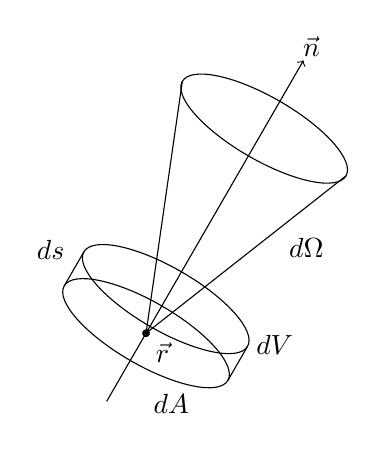
\begin{tikzpicture}
\begin{scope}[rotate=-30]
\fill[black] (0,0) circle [radius=0.05];
\draw[->] (0,-1) -- (0,4);
\draw(0,0) ellipse [x radius=1.2cm,y radius=0.4cm];
\draw(0,0.5) ellipse [x radius=1.2cm,y radius=0.4cm];
\draw(+1.2,0.5) -- (+1.2,0);
\draw(-1.2,0.5) -- (-1.2,0);
\draw(0,3) ellipse [x radius=1.2cm,y radius=0.4cm];
\draw(0,0) -- (-1.2,3);
\draw(0,0) -- (+1.2,3);
\draw (0,4.2) node {$\vec n$};
\draw (0,0) node[below right] {$\vec r$};
\draw (1.3,0.3) node[above right] {$dV$};
\draw (0.6,-0.4) node[below] {$dA$};
\draw (-1.2,0.25) node[above left] {$ds$};
\draw (0.8,2) node[below right] {$d\Omega$};
\end{scope}
\end{tikzpicture}
\end{center}
\caption{The geometry of the derivation of the transfer equation.}
\label{fig-transfer-equation}
\end{figure}

\newslide

Consider Figure \ref{fig-transfer-equation}, which shows the
volume $dV$ formed by sweeping an area $dA$ centered on
$\vec r$ thought a length $ds$ parallel to $\vec n$ which is
perpendicular to $dA$. Consider now the evolution of the
energy carried by radiation that enters the volume in solid
angle $d\Omega$ centered on $\vec n$, in frequency interval
$(\nu,\nu+d\nu)$, and in time interval $(t,d+dt)$. From the
definition of specific intensity, the energy that enters is
\begin{align}
I_\nu(\vec r,\vec n,\nu,t)\,dA\,d\Omega\,d\nu\,dt.
\end{align}
From the definition of the emissivity, the energy
added by emission in the volume, in the same intervals of
solid angle, frequency, and time, is
\begin{align}
j_\nu(\vec r,\vec n,\nu,t)\,dV\,d\Omega\,d\nu\,dt.
\end{align}
From the definition of the extincion coefficient, the energy
removed by extinction in volume, in the same intervals of
solid angle, frequency, and time, is
\begin{align}
\chi(\vec r,\vec n,\nu,t) I_\nu(\vec r,\vec n,\nu,t)\,dV\,d\Omega\,d\nu\,dt.
\end{align}
Finally, again from the definition of the specific
intensity, the energy that leaves the volume, in the same
intervals of solid angle and frequency but in the time
interval $(t + ds/c, t + ds/c + dt)$ is
\begin{align}
I_\nu(\vec r + \vec n ds, \vec n,\nu,t + ds/c)
\,dA\,d\Omega\,d\nu\,dt.
\end{align}
The time interval is retarded by $ds/c$ to account for the
time the photons take to traverse the volume.

\newslide

Conservation of energy gives
\begin{multline}
I_\nu(\vec r + \vec n ds, \vec n,\nu,t +
 ds/c)
 =\\
I_\nu(\vec r,\vec n,\nu,t) 
+ j_\nu(\vec r,\vec n,\nu,t)\,ds
- \chi(\vec r,\vec n,\nu,t) I_\nu(\vec r,\vec n,\nu,t)\,ds.
\end{multline}
Rearranging and letting $ds \rightarrow 0$, yields
\begin{align}
\frac{\partial I_\nu}{\partial s}
+ \frac{1}{c} \frac{\partial I_\nu}{\partial t}
= j_\nu -\chi I_\nu,
\end{align}
in which $\partial I_\nu/\partial s$ is the spatial
derivative along the path of the ray. We will normally treat
the case in which $I_\nu$ is independent of time, in which
case we can write this equation as
\begin{align}
\frac{d I_\nu}{ds}
= j_\nu -\chi I_\nu.
\end{align}
Note that in the absence of interaction with matter, that is, when the
emissivity and extinction coefficients are both zero, the specific
intensity is conserved, as we expect.

\newslide

The equation of radiation transfer becomes easier to manipulate if we
change variables by introducing a quantity known as the optical depth.
We can define the optical depth $\tau$ by
\begin{align}
\frac{d\tau}{ds} \equiv \chi
\end{align}
along with a suitable boundary condition (e.g., $\tau = \tau_0$
at $s = 0$). With this boundary condition we can integrate
this equation to give
\begin{align}
\tau(s) &= \tau_0 + \int_0^s ds'\:\chi(s').
\end{align}
Since $\chi = l^{-1}$, the optical depth is also given by
\begin{align}
\tau(s) &= \tau_0 + \int_0^s \frac{ds'}{l(s')},
\end{align}
and so we can see that the optical depth measures distance in units of the mean free path. The equation of
radiation transfer becomes
\begin{align}
\frac{dI_\nu}{d\tau} = \frac{j_\nu}{\chi} - I_\nu.
\end{align}

\newslide

We can simplify this further by defining the source function $S_\nu$
as
\begin{align}
S_\nu \equiv \frac{j_\nu}{\chi} = j_\nu l
\end{align}
The emissivity $j_\nu$ measures in some sense the emission per cm along
the beam; since $l = \chi^{-1}$, the source function $S_\nu$ measures the emission per mean free path along
the beam. However, since each mean free path is equal to a unit of optical depth, the source function $S_\nu$ also measures the emission per unit of optical depth along the beam.

In terms of the optical depth $\tau$ and the source function $S_\nu$, equation of radiation transfer is
\begin{align}
\frac{dI_\nu}{d\tau} = S_\nu - I_\nu.
\end{align}
This is the fundamental equation of radiation transfer. It is a
first-order differential equation that describes how the specific
intensity changes as a result of the interaction of the radiation field
with matter. 

\newslide

It's worth considering for a moment the role of the source function in
the equation of radiation transfer. If $S_\nu > I_\nu$, then
$dI_\nu/d\tau$ is positive and $I_\nu$ grows along the ray; if
$S_\nu < I_\nu$, then $dI_\nu/d\tau$ is negative and $I_\nu$
decreases along the ray; and if $S_\nu =
I_\nu$ then $dI_\nu/d\tau$ is zero and $I_\nu$ does not change along
the ray. Thus, we see that the equation of radiation transfer acts to force $I_\nu$
to approach $S_\nu$. It does this by transferring energy either from matter to radiation or from radiation to matter, according to whether $S_\nu$ is larger or smaller than $I_\nu$.

\newslide

\section{Formal Solution}

We can obtain the formal solution to the equation of radiation transfer
by moving terms in $I_\nu$ to one side and multiplying by the
integrating factor $e^{\tau}$, obtaining
\begin{align}
e^{\tau} \frac{dI_\nu}{d\tau} + e^{\tau} I_\nu =
e^{\tau} S_\nu.
\end{align}
This can be integrated, and the constant of integration
fixed by the the boundary conditions $I_\nu(\tau_0)$, to
give
\begin{align}
\Bigl[e^t I_\nu(t)\Bigr]_{\tau_0}^{\tau} =
\int_{\tau_0}^{\tau}\!\!\!dt\:e^t S_\nu(t),
\end{align}
and ultimately
\begin{align}
I_\nu(\tau) &=
e^{(\tau_0-\tau)}I_\nu(\tau_0) + \int_{\tau_0}^{\tau}\!\!\!dt\:e^{(t-\tau)}S_\nu(t).
\end{align}
Thus, if we know the specific intensity of an incident ray,
the value of the source function all along its path, and the
value of $\chi$ all along its path (to calculate
$\tau$), we can directly calculate the specific intensity
of the emergent ray.

\newslide

To better understand the form of the formal result, we can
make the subsitutions $\Delta\tau = \tau -
\tau_0$ and $t' = \tau - t$, to give
\begin{align}
I_\nu(\tau) = e^{-\Delta\tau}I_\nu(\tau_0)
+
\int_0^{\Delta\tau}\!\!\!dt'\:e^{-t'}S_\nu(\tau -
t').
\end{align}
Thus, the intensity is given by the incident intensity $I(\tau_0)$
diminished by a factor of $e^{-\Delta\tau}$, the negative
exponential of the optical depth to the point of incidence, plus the
integral along the path of the contributions to the intensity
$S_\nu(\tau - t')$ diminished by a factor of $e^{-t'}$, again the
negative exponential of the optical depth to the point making the
contribution. The factor of $e^{-t'}$ is characteristic of radiation
transfer problems. Mathematically, it arise because of the $-I_\nu$ term
in the equation for radiation transfer. Physically, it expresses the
fact that a the distance traveled by a photon has an exponential
distribution, so that a fraction $1/e$ of the radiation making up the
specific intensity is extinguished for each mean free path traveled.
This point is explored more fully in Problem
\ref{problem-optical-depth}.

This expression is known as the formal solution because it is a solution
for $I_\nu$ in terms of $S_\nu$. The source function is the ratio of the
emissivity $j_\nu$ and extinction coefficient $\chi$, and so depends
on the state of matter. However, as the interaction of radiation with
matter determines the state of matter, the source function $S_\nu$
depends on the specific intensity $I_\nu$. Thus, effectively, the
specific intensity appears in the integral, and so the formal solution
is an implicit solution.

\newslide

\section{Derivation in Plane-Parallel Symmetry}

When working with plane-parallel symmetry, we often use a
different definition of optical depth, which has
\begin{align}
\frac{d\tau}{dz} \equiv - \chi.
\end{align}
This definition measures the optical depth parallel to the $z$ axis,
regardless of the angle of the path, and furthermore measures it into
the atmosphere, so that $\tau$ increases as $z$ decreases.
Conventionally $z$ increases outwards in the atmosphere, and so the
minus sign in the definition acts so that the optical depth increases
inwards. The conventional boundary condition is that $\tau = 0$
outside the atmosphere (i.e., at $z = +\infty$). 

The lengths parallel to the $z$ axis are shorter than lengths along the
path by a factor of $dz/ds = \cos\theta = \mu$, where $\theta$ is the angle
between the path and the $z$ axis. Thus, we have $ds = dz/\mu
= -d\tau / \mu \chi$.
The equation of radiation transfer now becomes
\begin{align}
\mu \frac{dI_\nu}{dz}
= - \chi I_\nu + j_\nu,
\end{align}
or
\begin{align}
\mu \frac{dI_\nu}{d\tau}
= I_\nu - S_\nu.
\end{align}

\newslide

\section{Formal Solution in Plane-Parallel Symmetry}

In plane-parallel symmetry, the formal solution becomes
\begin{align}
I_\nu(\tau,\mu) &=
e^{(\tau-\tau_0)/\mu}I_\nu(\tau_0,\mu) + 
\int_{\tau}^{\tau_0}\!\frac{dt}{\mu}\:e^{(\tau-t)/\mu}S_\nu(t).
\end{align}
If we have a semi-infinite plane-parallel atmosphere (i.e.,
it is unbounded as $z \rightarrow -\infty$ and $\tau
\rightarrow \infty$) and has no incident intensity from
above (i.e., $I_\nu(0,\mu) = 0$ for $\mu \le 0$), then the
intensity is given for $\mu > 0$ by
\begin{align}
I_\nu(\tau,\mu) = 
\int_{\tau}^\infty\!\frac{dt}{\mu}\: e^{(\tau -
t)/\mu} S_\nu(t),
\end{align}
and for $\mu < 0$ by
\begin{align}
I_\nu(\tau,\mu) = 
\int_{\tau}^0\!\frac{dt}{\mu}\: e^{(\tau -
t)/\mu} S_\nu(t).
\end{align}
The first terms in the formal solution disappear for the
case $\mu > 0$ as $e^{-\tau/\mu}I_\nu(\tau)
\rightarrow 0$ as $\tau \rightarrow \infty$ for any
finite $I_\nu(\tau)$. It disappears for the case $\mu
< 0$ by the boundary condition $I_\nu(0,\mu) = 0$ for $\mu
< 0$.

These results again become clearer and more symmetrical if
we make the substitutions $t' = t-\tau$ for $\mu
> 0$ and $t' =
\tau-t$ for $\mu < 0$, and also use $|\mu|$ to avoid confusion over
the sign of $\mu$. The formal solutions is 
then given by
\begin{align}
I_\nu(\tau,\mu) =
\begin{cases}
\int_0^\infty\,\,\frac{dt'}{|\mu|}\: e^{-t'/|\mu|}
S_\nu(\tau+t')
&\mbox{for $\mu > 0$,}\\
\int_0^{\tau}\!\frac{dt'}{|\mu|}\: e^{-t'/|\mu|}
S_\nu(\tau-t')
&\mbox{for $\mu < 0$.}
\end{cases}
\end{align}
Thus, the intensity is given by the integral along the path
to the appropriate boundary of the contribution to the
intensity $S_\nu$ diminished by a factor $e^{-t'/|\mu|}$.

An important special case is the emergent intensity
$I_\nu(0,\mu)$ for $\mu > 0$ from a semi-infinite
atmosphere, which is given by
\begin{align}
I_\nu(0,\mu) = \int_0^\infty\!\frac{dt}{\mu}\:e^{-
t/\mu} S_\nu(t).
\end{align}
The emergent flux $F_\nu(0)$ is given by
\begin{align}
F_\nu(0) = 2\pi \int_0^1\!\!\!d\mu\int_0^\infty\!\!\!dt\:e^{-
t/\mu} S_\nu(t).
\end{align}
Thus, given $S_\nu(\tau)$, we can calculate the emergent flux. Much of the effort in atmospheres is therefore dedicated to finding $S_\nu(\tau)$ and $\tau(z)$.

%Note that $I_\nu(0,\mu)$ is the Laplace transform of $S_\nu(\mu t)$; this can be useful sometimes in understanding the dependence of the emergent flux on the source function and, occasionally, in seeking solutions.
\newslide

\section{The Schwarzschild Equation}

We can write the mean intensity $J_\nu(\tau)$ in terms
of the upwards and downwards mean intensities
$J_\nu^+(\tau)$ and $J_\nu^-(\tau)$ as
\begin{align}
J_\nu(\tau) = \frac{1}{2} \left[J_\nu^+(\tau) + J_\nu^-(\tau)\right],
\end{align}
where
\begin{align}
J_\nu^+(\tau) \equiv\int_{0}^{+1}\!\!\!d\mu\:I_\nu(\tau,\mu),
\end{align}
and
\begin{align}
J_\nu^-(\tau) \equiv\int_{-1}^{0}\!\!\!d\mu\:I_\nu(\tau,\mu).
\end{align}
We can use the formal solution for $I_\nu(\tau,\mu)$ in
these definitions to obtain
\begin{align}
J_\nu^+(\tau)=
\int_0^{+1}\!\!\!d\mu
\int_{\tau}^\infty\!\!\frac{dt}{\mu}\:e^{(\tau-t)/\mu} S_\nu(t),
\end{align}
and
\begin{align}
J_\nu^-(\tau)=
\int_{-1}^{0}\!\!\!d\mu
\int_{\tau}^0\!\!\frac{dt}{\mu}\:e^{(\tau-t)/\mu} S_\nu(t).
\end{align}
If we make the substitutions $w = +\mu^{-1}$ in the
expression for $J_\nu^+$ and $w = -\mu^{-1}$ in the
expression for $J_\nu^-$, we obtain
\begin{align}
J_\nu^+(\tau)=
\int_{\tau}^\infty\!\!\!dt\:
S_\nu(t)
\int_1^\infty\!\!\frac{dw}{w} e^{w(\tau-t)},
\end{align}
and
\begin{align}
J_\nu^-(\tau)=
\int_0^{\tau}\!\!\!dt\:
S_\nu(t)
\int_1^\infty\!\!\frac{dw}{w} e^{w(t-\tau)}.
\end{align}
The integrals over $w$ have the form of the first exponential
integral $E_1$ \citep[pp.\ 228-231]{Abramowitz-1972}, where
$E_n$ is defined by
\begin{align}
E_n(x) &\equiv \int_1^\infty \!\!\!dw\: w^{-n}e^{-xw}.
\end{align}
Thus
\begin{align}
J_\nu^+(\tau)=
\int_{\tau}^\infty\!\!\!dt\:
S_\nu(t)
E_1(t-\tau),
\end{align}
and
\begin{align}
J_\nu^-(\tau)=
\int_0^{\tau}\!\!\!dt\:
S_\nu(t)
E_1(\tau-t).
\end{align}
However, given the ranges of the two integrals over
$t$, in both expressions the argument to the
exponential integral is non-negative, so we can write it as
$|t-\tau|$. After this, the two integrands are
identical, and we can combine the integrals to give
\begin{align}
J_\nu(\tau) = \frac{1}{2} \int_0^\infty\!\!\!dt\:
S_\nu(t)
E_1(|t-\tau|).
\end{align}
This is known as the Schwartzschild equation \cite{Schwarzschild-1914}. 

%\begin{figure}
%\includefigure{schwarzschild-equation}
%\caption{The kernel $E_1(|t - \tau|)/2$ of the Schwarzschild equation.}
%\label{figure-schwarzschild-equation}
%\end{figure}
%
%It is worth considering the Schwarzschild equation more closely. It
%states that the mean intensity $J_\nu(\tau)$ is given by convolving
%the source function $S_\nu(t)$ with the kernel
%\begin{align}
%\frac{1}{2}E_1(|t - \tau|)
%&=
%\frac{1}{2}
%\int_1^\infty \!\!\!dw\: \frac{e^{-|t-\tau|w}}{w}.
%\end{align}
%Figure~\ref{figure-schwarzschild-equation} shows this kernel. 
%The limiting cases of $E_1$ are $E_1(x) \rightarrow -\gamma -\ln x$ as $x
%\rightarrow 0$ where $\gamma$ is Euler's constant ($0.57721\ldots$)
%and $E_1(x)
%\rightarrow e^{-x}/x$ as $x\rightarrow \infty$
%\citep[p.\ 229]{Abramowitz-1972}. 
%Thus, the kernel is strongly peaked at $t = \tau$, but falls off
%very rapidly. It is easy to show that the contribution to $J_\nu$ from
%the interval $(\tau-\epsilon,\tau+\epsilon)$ is $\epsilon
%S_\nu(\tau) + O(\epsilon^3)$, provided $S_\nu$ is sufficiently
%smooth, and so despite the logarithmic divergence in the kernel, $J_\nu$ remains
%finite. For normal source functions, the dominant contribution to
%$J_\nu(\tau)$ comes from $S_\nu$ in the vicinity of $\tau$,
%although we cannot completely ignore contributions from further away.

For conciseness, we can define an operator $\Lambda_1$, such
that
\begin{align}
\Lambda_1(f) \equiv \frac{1}{2} \int_0^\infty\!\!\!dt\:
f(t)
E_1(|t-\tau|).
\end{align}
With this notation, the Schwartzschild equation becomes
\begin{align}
J_\nu(\tau) = \Lambda_1(S_\nu).
\end{align}
The $\Lambda$ operator is almost ubiquitous in the development of
numerical solutions to the equation of radiative transfer.

\newslide

\section{The Milne Equation}

In a similar manner to the Schwarzschild equation, we can obtain the
Milne equation \cite[p.\ 130]{Milne-1930},
\begin{align}
H_\nu(\tau) &= 
 \frac{1}{2}\int_{\tau}^\infty\!\!\!dt\: S_\nu(t) E_2(t - \tau)
 - 
\frac{1}{2} \int_0^{\tau}\!dt\: S_\nu(t) E_2(\tau - t)\\
&\equiv \Lambda_2(S_\nu).
\end{align}
